\documentclass[12pt,a4paper]{article}

% Кодування/мови — в такому порядку
\usepackage[utf8]{inputenc}
\usepackage[T2A]{fontenc}
\usepackage[ukrainian]{babel}
\usepackage{cmap}

\usepackage{geometry}
\geometry{left=2cm,right=2cm,top=2cm,bottom=2cm}

\usepackage{graphicx}
\usepackage{array,multirow,booktabs,makecell}
\usepackage{caption}
\renewcommand{\thetable}{\arabic{table}}
\captionsetup[table]{name=Таблиця}

\usepackage{amsmath}
\usepackage{pdflscape}
\usepackage{xcolor}

\newcommand{\g}{\cellcolor{gray!25}} % коротке позначення сірого

% Гіперпосилання — тримай наприкінці пакетів, з unicode
\usepackage[unicode]{hyperref}

\renewcommand\cellalign{tc}
\renewcommand\theadalign{cc}
\newcommand{\addh}{\rule{0pt}{3.8ex}} % ДОДАТКОВА ВИСОТА РЯДКА (лише де потрібно)
\renewcommand{\arraystretch}{1.25}

\begin{document}

    \begin{titlepage}

        % Картинка шапки (по центру, з відступом від верху)
        \begin{center}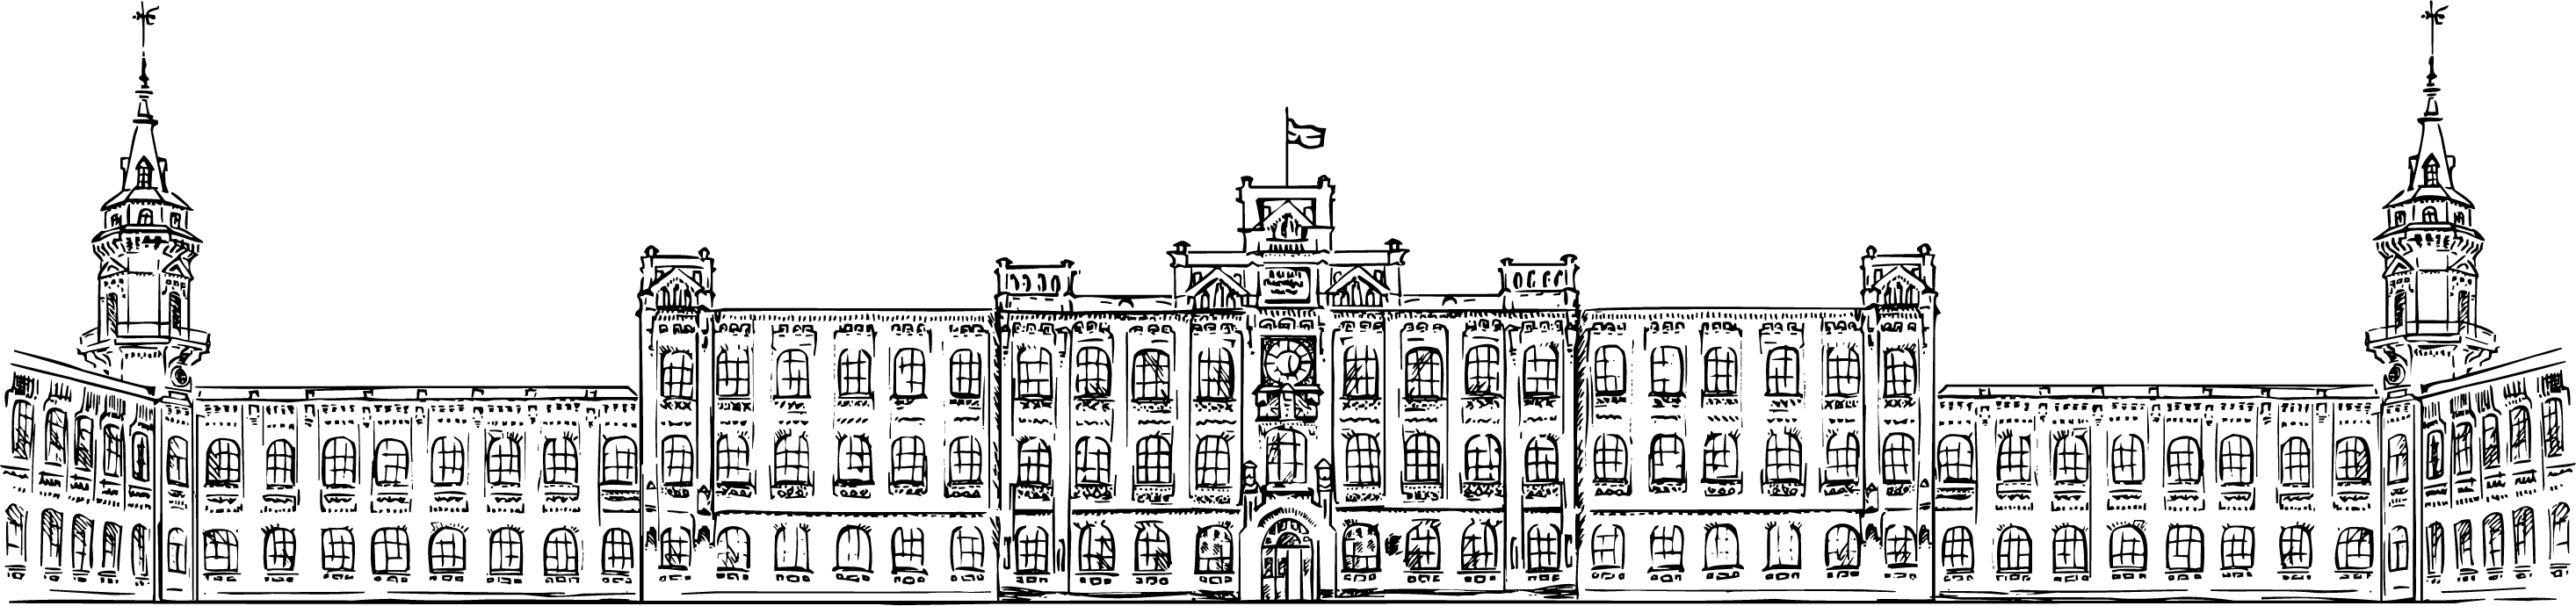
\includegraphics[width=0.7\textwidth]{../../../TITLES/letterhead.png}\end{center}

        \begin{center}
            \large Національний технічний університет України\\
            «Київський політехнічний інститут імені Ігоря Сікорського»\\[1em]
            Факультет інформатики та обчислювальної техніки\\
            Кафедра обчислювальної техніки
        \end{center}

        \vfill

        \begin{center}
            \textbf{\LARGE Теорія електричних кіл та сигналів}\\[2em]
            \textbf{\Large Лабораторна робота №7}\\[0.5em]
            «Дослідження перехідних процесів у лінійних електричних колах з послідовним з'єднанням RL елементів»
        \end{center}

        \vfill

        \begin{flushright}
            Виконав: студент 2 курсу ФІОТ, гр. ІО-41\\
            \textit{Давидчук А.~М.}\\[1em]
            Перевірив: \textit{Лободзинський В.~Ю.}
        \end{flushright}

        \vfill

        \begin{center}Київ --- 2025\end{center}

    \end{titlepage}

    \noindent
    \textbf{\underline{Тема:}} «Дослідження перехідних процесів у лінійних електричних колах з послідовним з'єднанням RL елементів».

    \vspace{1em}

    \noindent
    \textbf{\underline{Мета:}} Дослідження перехідних процесів в електричних колах постійного струму при
послідовному з'єднанні резистивно-індуктивних (RL) елементів.

    \begin{center} \textbf{\Large Практична частина} \end{center}

    Усі розрахунки було проведено за допомогою мови програмування Python (вихідний код додано разом із звітом).

    \vspace{1em}

    Моя група: IО-41, мiй порядковий номер у групi: 6. Звiдси $N = 6, S = 1$.

    Загальна структурна схема електричного кола:

    \begin{figure}[h!]
        \renewcommand{\thefigure}{\arabic{figure}} % робимо "3.1", "3.2" і т.д.
        \centering
        
\includegraphics[width=0.5\textwidth]{s0.png}
        \caption{Структурна схема електричного кола}
    \end{figure}

    \vspace{1em}

    Розраховані параметри елементів:

    \begin{table}[h!]
        \centering
        \begin{tabular}{|c|c|c|c|}
            \hline
            $E,\,\text{В}$ & $R,\,\text{Ом}$ & $L,\,\text{Гн}$ & $R_k,\,\text{Ом}$ \\
            \hline
            11& 216 & $0{,}7$ & 116 \\
            \hline
        \end{tabular}
        \caption{Розраховані параметри елементів кола}
    \end{table}

    Розрахована постійна часу $\tau_1$ та перехідного процесу $T_{\text{пп}}$:

    \begin{table}[h!]
        \centering
        \begin{tabular}{|c|c|}
            \hline
            $\tau_1,\,\text{с}$ & $T_{\text{пп}},\,\text{с}$ \\
            \hline
            0{,}002108& 0{,}02108 \\
            \hline
        \end{tabular}
        \caption{Розрахована постійна часу та перехідного процесу}
    \end{table}

    На основі $T_{\text{пп}}$, розрахую частоту джерела напруги тактової частоти (генератор прямокутних хвиль):

    \[
    f = T_{\text{пп}}^{-1} \approx 48 \text{ Гц}
    \]

    \newpage

    На основі загальної структури електричного кола та попередньо розрахованих параметрів її елементів, побудую електричну схему у програмі Multisim:

    \begin{figure}[h!]
        \renewcommand{\thefigure}{\arabic{figure}} % робимо "3.1", "3.2" і т.д.
        \centering
        \includegraphics[width=1\textwidth]{scheme.pdf}
        \caption{Електрична схема у програмi Multisim}
    \end{figure}

    \noindent
    Отримуємо осцилограми $u_R(t), u_L(t)$:

    \begin{figure}[h!]
        \renewcommand{\thefigure}{\arabic{figure}} % робимо "3.1", "3.2" і т.д.
        \centering
        
\includegraphics[width=1\textwidth]{graph0.png}
        \caption{Осцилограми напруг на резисторі та на котушці індуктивності}
    \end{figure}

    \newpage

    Далі визначимо графічно значення $\tau$ при замиканні/розмиканні ключа (використовуватимемо графік $u_L(t)$):

    \begin{figure}[h!]
        \renewcommand{\thefigure}{\arabic{figure}} % робимо "3.1", "3.2" і т.д.
        \centering
        
\includegraphics[width=0.95\textwidth]{graph1.png}
        \caption{Значення $\tau = dx = x_2 - x_1$ при замиканні ключа}
    \end{figure}

    \begin{figure}[h!]
        \renewcommand{\thefigure}{\arabic{figure}} % робимо "3.1", "3.2" і т.д.
        \centering
        
\includegraphics[width=0.95\textwidth]{graph2.png}
        \caption{Значення $\tau = dx = x_2 - x_1$ при розмиканні ключа}
    \end{figure}

    Результати графічного обчислення $\tau$ зведемо до таблиці:

    \begin{table}[h!]
        \centering
        \begin{tabular}{|p{7cm}|p{7cm}|}
            \hline
            \centering $\tau$ при розмиканні ключа, с & \centering $\tau$ при замиканні ключа, с \tabularnewline
            \hline
            \centering $2,043 \cdot 10^{-3}$& \centering $2,1148 \cdot 10^{-3}$ \tabularnewline
            \hline
        \end{tabular}
    \end{table}

    \newpage

    Також із графіка визначимо $U_{L_y}$ та $U_{R_y}$:

    \begin{figure}[h!]
        \renewcommand{\thefigure}{\arabic{figure}} % робимо "3.1", "3.2" і т.д.
        \centering
        
\includegraphics[width=0.5\textwidth]{graph3.png}
        \vfil
        
\includegraphics[width=0.5\textwidth]{graph4.png}
        \caption{Значення $U_{L_y}$ та $U_{R_y}$}
    \end{figure}

    Тут

    \[
    U_{L_y} = 3{,}8939 \text{ В} \quad U_{R_y} = 7{,}1058 \text{ В}
    \]

    Звідси 

    \[
    R_k \approx 118{,}37 \text{ Ом}
    \]

    Далі будемо використовувати осцилограму $u_L(t)$ задля розрахунку значення складових аналітичних виразів $u_L(t), u_R(t)$ при замиканні та розмиканні ключа.
    Аналітичні вирази $u_L(t), u_R(t)$ при замиканні ключа:

    \[
    u_L(t) =
    \frac{ER_{k}}{R + R_{k}}
    + \frac{ER}{R + R_{k}}\, e^{-\dfrac{R + R_{k}}{L} t}.
    \]

    \[
    u_R(t) = Ri(t) = \frac{ER}{R + R_{k}} \left( 1 - e^{-\dfrac{R + R_{k}}{L} t} \right),
    \]

    де $E = 11$ В, $R = 216$ Ом, $R_k = 116$ Ом, $L = 0{,}7$ Гн. Побудую графіки:

    \begin{figure}[h!]
        \renewcommand{\thefigure}{\arabic{figure}}
        \centering
        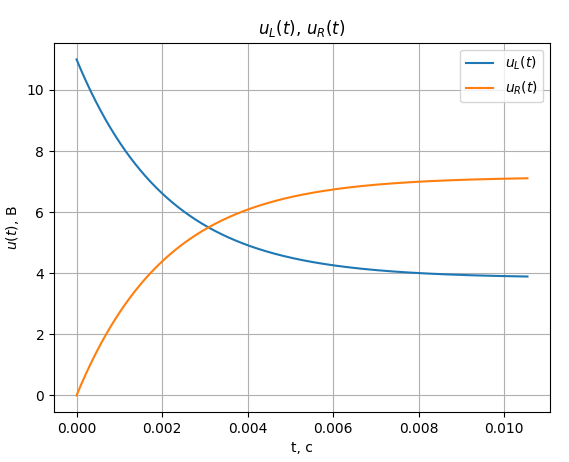
\includegraphics[width=0.5\textwidth]{graph5.png}
        \caption{Графік виразів $u_L(t)$ та $u_R(t)$ при замиканні ключа}
    \end{figure}

    Аналітичні вирази $u_L(t), u_R(t)$ при розмиканні ключа:

    \[
    u_L(t) = -\,\frac{ER}{R + R_{k}} \, e^{-\dfrac{R + R_{k}}{L} t}
    \]

    \[
    u_R(t) = \frac{ER}{R + R_{k}} \, e^{-\dfrac{R + R_{k}}{L} t}
    \]

    Побудую графіки:

    \begin{figure}[h!]
        \renewcommand{\thefigure}{\arabic{figure}}
        \centering
        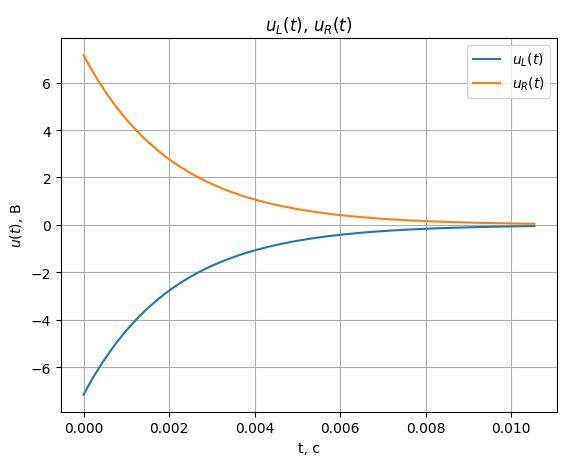
\includegraphics[width=0.5\textwidth]{graph6.png}
        \caption{Графік виразів $u_L(t)$ та $u_R(t)$ при розмиканні ключа}
    \end{figure}

    На основі осцилограм напруги на $u_R(t)$ (скільки $u_R(t) \propto i(t)$, форма осцилограми відповідає струму.) та аналітичних розрахунків перевіримо виконання 
    закону комутації для індуктивності. Відомо, що струм через індуктивність не може 
    змінюватися стрибком у момент перемикання ключа, тобто має виконуватися умова:
    \[
    i_L(0^-) = i_L(0^+).
    \]

    З осцилограми видно, що лівобічна та правобічна границя струму $i(t)$ (напруги $u_R(t)$) є однаковою (графік не має стрибків при $t=0$). Оскільки значення до та після комутації збігаються,
    закон комутації для струму через індуктивність виконується.

    \vspace{1em}

    \noindent
    \textbf{\underline{Висновок:}} У ході виконання лабораторної роботи було досліджено перехідні процеси у
    лінійному електричному колі з послідовним з'єднанням резистора та
    індуктивності. На основі розрахованих параметрів елементів кола побудовано
    осцилограми напруг $u_R(t)$ та $u_L(t)$, визначено сталу часу
    $\tau_1$, а також графічно та аналітично підтверджено основні закономірності
    процесів у RL-колах.

    За результатами графічних вимірювань значення сталої часу при
    замиканні та розмиканні ключа узгоджуються між собою та з теоретичним
    значенням, що підтверджує правильність моделі перехідного процесу.
    Порівняння експериментальних значень $U_{L_y}$ і $U_{R_y}$ дало можливість
    визначити еквівалентний опір $R_k$, який також узгоджується з очікуваним.

    Побудовані аналітичні залежності $u_L(t)$ та $u_R(t)$ у режимах
    заряджання та розряджання струму повністю збігаються з формою осцилограм,
    що свідчить про коректність теоретичного опису RL-ланцюга.

    Окремо було перевірено виконання закону комутації для індуктивності.
    Встановлено, що струм через індуктивність у момент перемикання ключа не
    змінюється стрибком:
    \[
    i_L(0^-) = i_L(0^+).
    \]
    З осцилограми напруги на резисторі $u_R(t)$ видно, що значення струму до і
    після моменту комутації збігаються, а графік не має розривів у точці
    $t=0$. Це підтверджує фізичний принцип неперервності струму в
    індуктивності та відповідність кола закону комутації.

    Таким чином, у ході роботи підтверджено теоретичні властивості RL-ланцюга,
    проведено аналітичне та графічне дослідження перехідних процесів, а також
    експериментально перевірено виконання закону комутації для індуктивності.

\end{document}